\documentclass[11pt]{article}
\usepackage[margin=1in]{geometry}
\usepackage{booktabs}
\usepackage{graphicx}
\usepackage{xcolor}
\usepackage{amsmath}
\usepackage{hyperref}
\hypersetup{colorlinks=true, linkcolor=teal, urlcolor=teal}
\newcommand{\win}[1]{\textbf{#1}}
\newcommand{\loss}[1]{#1}
\setlength{\parskip}{0.35em}
\setlength{\emergencystretch}{2.5em}

\title{\textbf{SMOR: Technical Notes}\\[2pt]
\large Utilization and acquisition as one value-estimation problem}
\author{Van Thanh Pham}
\date{\today}

\begin{document}
\maketitle
\vspace{-2.2em}

\section{Motivation}
Robot-learning datasets are assembled from heterogeneous sources (teleop devices, operators,
machine-generated rollouts). Two questions are usually studied apart. \emph{Utilization}: given a
fixed dataset, how to weight each source---online reweighting / confidence, as in CAIL and
our SMOR. \emph{Acquisition}: given a budget $B$, what mixture $p$ to collect, and
how the optimum $p^\ast$ changes with scale---a data-scaling law. We argue they are \emph{one}
problem: both read the same per-source value signal, at two scales. A cheap pilot utilization pass
yields a confidence $\beta$ and hypergradient $h$ per source; acquisition extrapolates that value
over quantity ($\beta$ at pilot scale $\approx p^\ast$ at the target budget). The linchpin is the
\emph{outer-loss design}: the signal is trustworthy only if utilization's outer objective is
aligned with the true deployment goal (task return), not a proxy that matches a privileged
``clean'' source.

\section{Setup}
The learner is fixed across all methods---behavior cloning (MLP, Adam)---to isolate the
\emph{weighting} mechanism. Weighting methods: \texttt{uniform}, \texttt{only:source},
\texttt{static\_quality} (best-labelled source), CAIL (one-step hypergradient $K{=}1$,
ranking outer loss), SMOR (curvature-aware $K{>}1$). Outer losses: open-loop
\texttt{ValidationLoss}/\texttt{CAILRanking}, and closed-loop \texttt{ClosedLoopRolloutReturn} with
REINFORCE/GRPO/PPO estimators. The primary metric is closed-loop success / return,
not validation MSE. Data: \emph{official}---CAIL Ant-v2, Minari (D4RL-modern) MuJoCo, RoboMimic
(robosuite); \emph{self-simulated}---point-mass and robosuite device-calibration (each source is one
systematic error, re-simulated).

\section{Utilization: two regimes of source heterogeneity}

\paragraph{Regime A --- sources differ by \emph{noise} (complementary): non-trivial mixture.}
Each source is the same task through a differently mis-calibrated device (rotation / anisotropic
gain / per-joint bias); no source dominates. Reweighting learns an \emph{interior} $\beta$ and, on
closed-loop success, beats uniform and CAIL (Table~\ref{tab:A}): on RoboMimic-lift the interior
mixture reaches $0.87$ success vs $0.20$ (uniform) and $0.40$ (CAIL), and with a genuinely harmful
``poison'' source $1.00$ vs $0.00$. On an easy task (point-mass) success saturates and uniform
already cancels the bias, so the advantage appears only in harder, compounding, closed-loop
settings.

\begin{table}[h]\centering\small
\caption{Regime A: complementary-noise sources. Success~$\uparrow$ (RoboMimic, 1 seed) / val~$\downarrow$ (point-mass).}
\label{tab:A}
\begin{tabular}{lccc}
\toprule
weights & Point-mass 3-dev (val$\downarrow$) & RM-lift 3-dev (succ$\uparrow$) & RM-lift good+poison (succ$\uparrow$)\\
\midrule
uniform            & 0.012 & \loss{0.20} & \loss{0.00}\\
best single source & 0.014 & 0.60 & 0.80\\
CAIL ($K{=}1$)     & 0.021 & 0.40 & ---\\
\textbf{SMOR} ($K{>}1$) & 0.021 & \win{0.87} & \win{1.00}\\
$\beta$ (SMOR)     & {[.17,.51,.33]} & interior & {[.27,.32,.41,0]}\\
\bottomrule
\end{tabular}
\end{table}

\begin{figure}[h]\centering
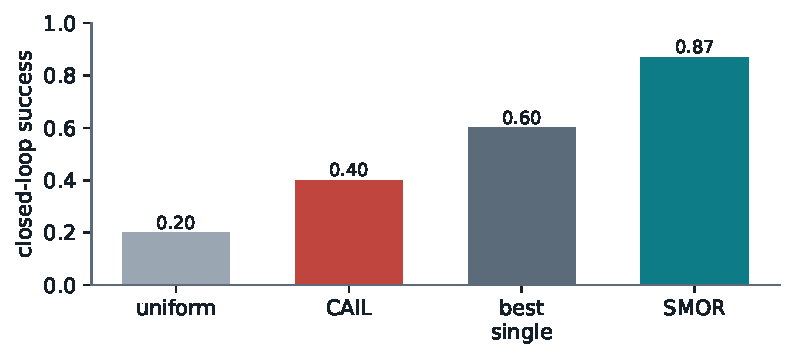
\includegraphics[width=0.62\textwidth]{fig_regimeA.pdf}
\caption{Regime A, RoboMimic-lift device sources: closed-loop success. The interior SMOR mixture
beats uniform and CAIL even where validation loss is a wash.}
\label{fig:A}
\end{figure}

\paragraph{Regime B --- sources differ by \emph{quality} (clean/dirty): trivial optimum, useful filter.}
When one source is strictly cleaner, the optimum \emph{collapses to a corner} (Table~\ref{tab:B}):
a ranking, not a mixture. But the learned weight is a reliable data filter---on the CAIL
Ant-v2 buffer it ranks demonstrations by their true return at Spearman $0.67$---which \emph{is} the
acquisition rule ``do not buy the dirty source.'' On these varying-optimality benchmarks curvature
$K{>}1$ (SMOR) $\approx$ one-step $K{=}1$ (CAIL): across CAIL Ant-v2 and modern Ant / HalfCheetah,
SMOR matches but does not beat CAIL. \emph{The contribution is therefore the outer loss, not the
curvature knob.}

\begin{table}[h]\centering\small
\caption{Regime B: RoboMimic quality tiers (official). Validation loss~$\downarrow$.}
\label{tab:B}
\begin{tabular}{lccc}
\toprule
weights & lift MH+MG & lift PH+MH & $\beta$ learned\\
\midrule
uniform & 0.044 & 0.039 & ---\\
\textbf{SMOR} & \textbf{0.023} & 0.030 & corner $\{$clean$\approx.99\}$\\
\bottomrule
\end{tabular}
\end{table}

\section{The novelty: outer-loss design}
CAIL's confidence loss rewards \emph{matching the ``expert'' source}, but the goal is task
return. Under BC covariate-shift, expert-only policies are brittle, so ``match expert'' diverges
from ``maximize return'' and the reweighter confidently loses to uniform (Table~\ref{tab:collapse}).
Replacing the proxy with the real return---estimated by a group-relative policy gradient
(GRPO, no critic) with a cosine-normalized hypergradient---realigns it and beats
uniform (Table~\ref{tab:grpo}). On robosuite manipulation (PH+MH+MG), SMOR+GRPO reaches success
$0.80$ vs $0.60$ for both uniform and CAIL, up-weighting \texttt{mg\_success} (machine
rollouts that \emph{actually succeed})---exactly what a quality ranking would discard.

\begin{table}[h]\centering\small
\begin{minipage}{0.49\textwidth}\centering
\caption{Misalignment: Minari (official), ranking outer loss. Return~$\uparrow$, 3 seeds.}
\label{tab:collapse}
\begin{tabular}{lccc}
\toprule
weights (ranking) & HC & Hop & Walk\\
\midrule
uniform & \win{2897} & 558 & \win{1145}\\
CAIL    & \loss{88}  & 552 & 610\\
SMOR    & \loss{154} & 591 & 631\\
\bottomrule
\end{tabular}
\end{minipage}\hfill
\begin{minipage}{0.49\textwidth}\centering
\caption{GRPO fix: Minari, closed-loop return. Return~$\uparrow$, 3 seeds.}
\label{tab:grpo}
\begin{tabular}{lccc}
\toprule
outer loss & HC & Hop & Walk\\
\midrule
uniform        & 1694 & 516 & 811\\
CAIL (ranking) & \loss{88} & 552 & 597\\
\textbf{SMOR+GRPO} & \win{2636} & 572 & \win{1264}\\
\bottomrule
\end{tabular}
\end{minipage}
\end{table}

\begin{figure}[h]\centering
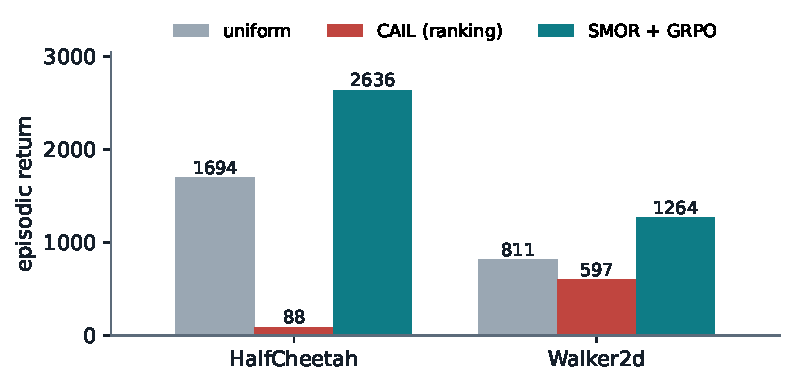
\includegraphics[width=0.68\textwidth]{fig_outerloss.pdf}
\caption{The outer loss decides the outcome (Minari, return, 3 seeds). CAIL's ranking loss
collapses to the brittle expert (return $\approx$ CAIL bar); the GRPO closed-loop return loss
recovers an interior mixture that beats uniform.}
\label{fig:outer}
\end{figure}

\noindent\textbf{Risk --- all-failed trajectories.} The return signal informs only when returns
\emph{vary}. With sparse reward and an under-trained policy (all rollouts fail), the advantage is
noise and the reweighter drifts: early runs put $0.48$--$0.74$ weight on the \emph{poison} source;
the $g_j$ normalization cut this to $0.20$, and dense reward / warm-up removes it. \emph{Power vs.\
the all-failed regime is the central design tension of the outer loss}, and motivates a value
baseline or curriculum warm-up.

\section{Acquisition: scaling law}
Fitting $(B,p)\!\to\!$ performance and extrapolating the optimal collection mixture $p^\ast(B)$: for
complementary-noise sources the optimum \emph{shifts with budget} (Table~\ref{tab:scale})---at
small budgets the precise source is preferred, at large budgets the unbiased source's diversity
wins. The fitted law extrapolates to held-out budgets (RMSE $0.016$, target-budget regret
$\le 0.0035$). For clean/dirty sources (RoboMimic PH vs MG, 90 runs) it is a flat \emph{dominance},
$p^\ast{=}1.0$ at every budget---the utilization filter \emph{is} the acquisition rule.

\begin{table}[h]\centering\small
\caption{Acquisition scaling: grid-optimal share of the unbiased source A vs.\ budget (point-mass, 210 runs).}
\label{tab:scale}
\begin{tabular}{lccccccc}
\toprule
budget $B$ & 50 & 100 & 200 & 400 & 800 & 1600 & 3200\\
\midrule
$p^\ast_A$ & 0.0 & 0.0 & 0.0 & \textbf{0.4} & \textbf{0.8} & 0.4 & 0.4\\
\bottomrule
\end{tabular}
\end{table}

\begin{figure}[h]\centering
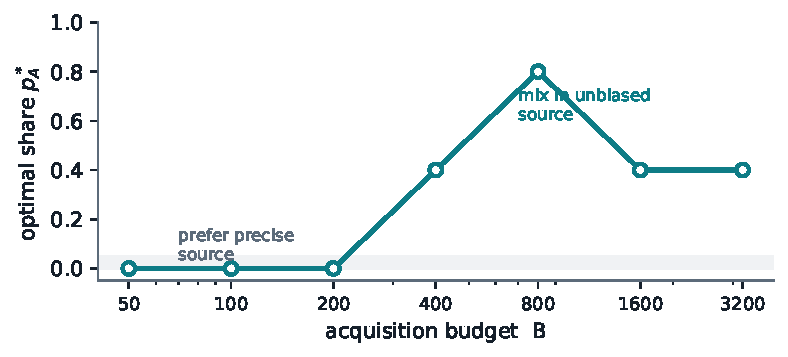
\includegraphics[width=0.62\textwidth]{fig_scaling.pdf}
\caption{Acquisition scaling (point-mass, 210 runs): the optimal share of the unbiased source rises
with budget---at small budgets buy the precise source, at large budgets mix in the unbiased one.}
\label{fig:scale}
\end{figure}

\section{Discussion}
Utilization and acquisition read the \emph{same} per-source value signal from opposite ends:
utilization measures value at the current pilot scale, acquisition extrapolates it over quantity.
In Regime A the signal is a mixture that moves with scale ($\beta$ at budget $B$ $\approx$ the
acquisition $p^\ast_B$); in Regime B it is a filter (utilization drops the dirty source
$\Rightarrow$ acquisition buys none of it). Both are trustworthy only when utilization's outer loss
is aligned---which is why the closed-loop / GRPO outer loss is the keystone connecting the two.

\paragraph{Status \& next.} $\sim$66 unit tests pass; datasets: CAIL Ant-v2, Minari
(halfcheetah/hopper/walker2d), RoboMimic (lift/square). RoboMimic-device and GRPO numbers are
1-seed / high-variance (policy-gradient); multi-seed runs are in progress. Next milestone: the
pilot~$\to$~acquisition bridge $F:\{\beta,h\}\!\to\!p^\ast(B)$---the scaling infrastructure
and reweighting-evidence object are in place. Codebase: this repository.

\end{document}
